% !TeX root = ../main.tex

\chapter{视觉行人追踪算法}

  计算机视觉中的行人追踪,主要包括密集跟踪方法,即基于行人检测和识别的追踪,以及稀疏跟踪方法,即基于目标动态的追踪。

  密集跟踪算法实际上并没有“跟踪”物体,而是在视频不同的时间点的一系列帧上扫描和检测物体的位置。由于每次的目标检测都是独立地在当前帧上进行的,所以每次检测时,都需要处理图像中的所有像素,所以用这种方法进行目标跟踪,计算量会比较大。此外,这种方法对分类器的要求也会较高,对于目标被遮挡的情况也不能很好地进行处理。

  由于目标的运动通常是连续的,我们可以根据物体的动态信息,对其可能的运动轨迹进行预测,并结合其上一帧所在位置和对当前帧的观察,得出其当前位置,这就是稀疏跟踪方法。由于已知物体在上一帧时的位置,所以对当前帧识别时,只需要检测上一帧物体所在位置附近的像素,这样一来,相对于密集跟踪方法,就减少了大量的计算。此外,由于我们结合了对物体运动的预测和观察来进行估计,在一些情况下准确度也会较高,例如,当目标发生较大形变或被暂时遮挡时,目标检测很可能下会直接失败,但由于在追踪时我们还记录了物体最后出现的位置和对其行为的预测,所以可以在一定准确程度上继续追踪物体。但在这种算法在物体速度较快时,由于不会进行全图扫描,也可能会失去对物体的追踪,当目标物暂时从视野中消失一段时间时,可能难以重新找回物体。

  比起基于检测的追踪,动态的目标追踪是在行人追踪任务中的主要方法,但行人检测在追踪算法中也是不可少的一环。下面将主要介绍在单张图像上的行人检测算法,和以此为基础的动态行人追踪。

\section{行人检测}

  经典的行人检测方法包括提取人工特征,将待检测目标作为正样本,不含该目标的图像作为负样本,使用分类器进行分类,再在全图上进行匹配。此外还有使用卷积神经网络(convolutional neural networks)来提取图像特征或进行分类的方法,是现在行人检测研究的主要方向,但深度神经网络在目前还难以同时兼顾准确和实时性要求,此处主要介绍人工特征和支持向量机(Support Vector Machines,SVM)、Boosting等分类器的使用。

\subsection{常用人工特征描述子}

  特征描述子是一种对图片的表示方法,它通过提取图片中的关键信息并丢弃多余信息来对图片信息进行简化。通常地,特征描述子算法可以将一个RGB三通道的图片转化成一个特征向量。为了做到精确地进行图像识别、目标检测,我们必须首先明确什么是关键的、有用的信息,什么是冗余信息。在目标检测领域,有以下的常用特征描述子被提出,并都有过较为成功的应用。

\subsubsection{颜色直方图}

  颜色特征是物体最为直观的特征之一,它具有旋转不变性,且不受目标的大小和形状的变化影响,在颜色空间中分布大致相同,从而具有较高的鲁棒性。颜色直方图是描述颜色特征最常用的描述子,它是是对目标表面颜色分布的统计,描述了不同色彩在图像中所占的比例,具有稳定性好、抗部分遮挡、计算方法简单和计算量小等优点。但它无法描述图像中颜色的局部分布及每种色彩所处的空间位置,即无法描述图像中的某一具体的对象或物体,只是对一个图像块的颜色分布的统计,所以也有其使用局限性。

  在行人检测领域,颜色直方图通常能够很好地描述行人的肤色或所着服饰的颜色,但在检测的时间段内,如果行人的衣着服饰发生改变,可能就会导致在接下来的时间检测失败。此外,杂乱的背景色和不同光照强度和颜色也会产生较大影响。

  颜色直方图可以基于不同的的颜色空间进行统计,其中,最常用的是RGB空间和HSV空间。数字图像一般都以RGB三通道形式进行存储,故这里首先以RGB空间为例。分别统计每个像素的R、G、B数值出现的频度,绘制出它们分别对应的直方图,以一张人物照片\ref{fig:ewan}为例,图\ref{fig:rgbhistogram}为其RGB分别对应的统计直方图。将直方图上每一个桶(bin)的高度作为一个分量,便可以得到一个统计向量,将R、G、B分别对应的直方图向量连接起来便可得到输入图像的RGB直方图特征向量。

\begin{figure}[htb]
  \centering
  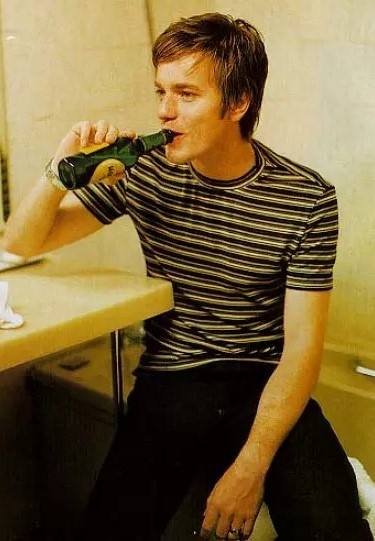
\includegraphics[width=0.3\textwidth]{ewan.jpg}
  \caption{原图}
  \label{fig:ewan}
\end{figure}

\begin{figure}[htb]
  \centering
  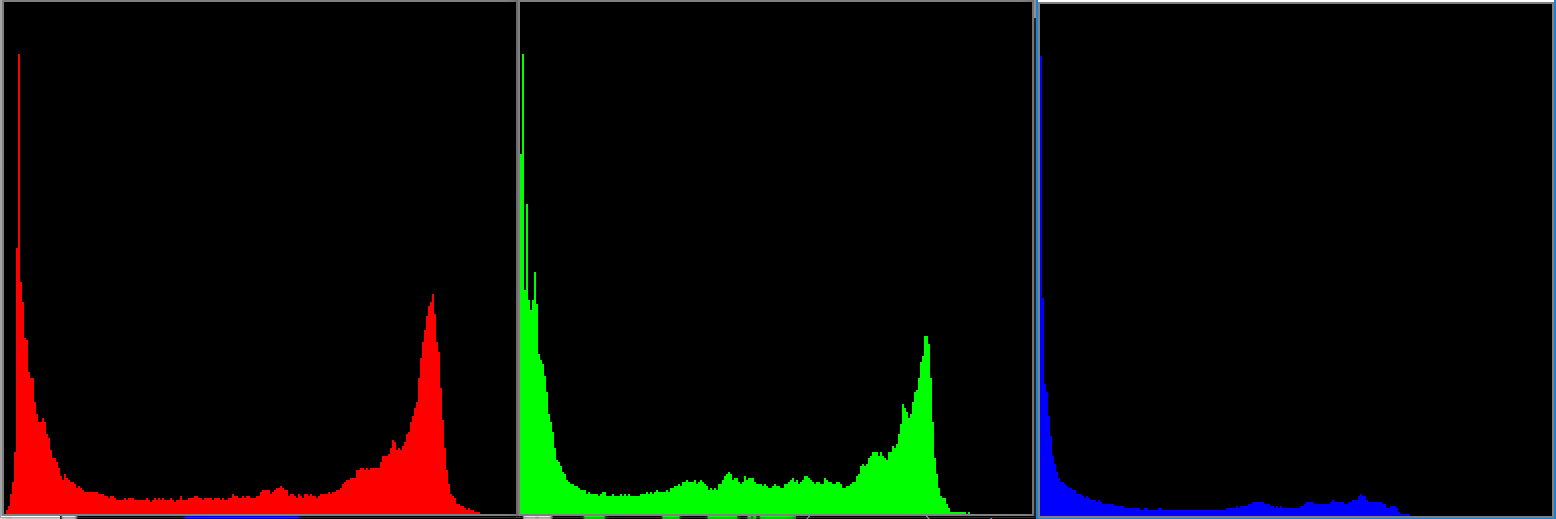
\includegraphics[width=0.6\textwidth]{rgb_histogram.png}
  \caption{左:B通道颜色直方图;中:G通道颜色直方图;右:R通道颜色直方图}
  \label{fig:rgbhistogram}
\end{figure}

  虽然RGB图像被如此普遍地使用,但以RGB直方图作为图片的特征描述子却有一些缺点。首先,RGB这三个重要的分量取值和其所生成的颜色之间的联系并不直观,即两种颜色在RGB空间中的距离无法描述它在人眼中的直觉色差。此外,使用RGB直方图的检测器容易受局部光照变化的影响而产生错误。所以在计算机视觉中,相比起RGB颜色空间,更常采用HSV颜色空间来表示颜色。HSV是一种将RGB色彩空间中的点在圆柱坐标系中的表示方法,相对于RGB,它能够更加直观地表示色彩的明暗、色调以及饱和度,方便对于不同颜色进行对比。此外,由于HSV单独提取了颜色的明暗,也可以一定程度上抵抗光照明暗带来的影响。\citet{sural2002segmentation}的实验显示,使用HSV直方图进行行人识别的结果比起RGB直方图可以有明显提高。

  HSV即色相(Hue)、饱和度(Saturation)、亮度(Value)。色相即表示物体的颜色名,取一个$0^{\circ}$到$360^{\circ}$的标准色轮,按照该颜色位置的角度来度量色相,即颜色点在圆柱坐标系中所在坐标的$\varphi$分量;饱和度是指颜色的强度或纯度,表示色相中灰色分量所占的比例,即圆柱坐标系的$\rho$分量;亮度是颜色的相对明暗程度,即在圆柱坐标系中的$z$分量。这些颜色坐标一般都落在圆柱坐标系的一个圆锥体中,如图\ref{fig:hsv}所示。

\begin{figure}[htb]
  \centering
  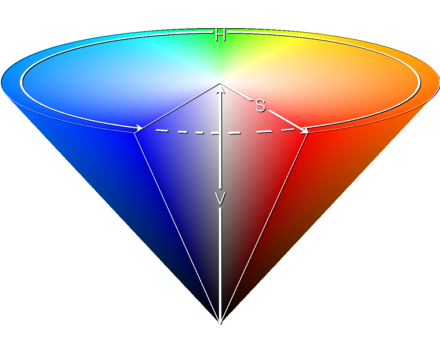
\includegraphics[width=0.3\textwidth]{hsv.png}
  \caption{HSV模型可以使用圆柱坐标系中的一个圆锥形子集表示}
  \label{fig:hsv}
\end{figure}

  在计算HSV直方图时,需要首先把RGB空间坐标映射到HSV空间。给定$(r,g,b)$分别是一个颜色的红、绿、蓝坐标,它们的值是在0到1之间的实数,$max$为$r$,$g$和$b$之中的最大值,$min$为其中的最小值,则从$(r,g,b)$到$(h,s,v)$的转换公式如下:\cite{foley1982fundamentals}

$$h={\begin{cases}0^{\circ }&{\mbox{if }}max=min\\60^{\circ }\times {\frac  {g-b}{max-min}}+0^{\circ },&{\mbox{if }}max=r{\mbox{ and }}g\geq b\\60^{\circ }\times {\frac  {g-b}{max-min}}+360^{\circ },&{\mbox{if }}max=r{\mbox{ and }}g<b\\60^{\circ }\times {\frac  {b-r}{max-min}}+120^{\circ },&{\mbox{if }}max=g\\60^{\circ }\times {\frac  {r-g}{max-min}}+240^{\circ },&{\mbox{if }}max=b\end{cases}}$$

$$s={\begin{cases}0,&{\mbox{if }}max=0\\{\frac  {max-min}{max}}=1-{\frac  {min}{max}},&{\mbox{otherwise}}\end{cases}}$$

$$
v=max
$$

  HSV直方图的计算与RGB类似,只是将颜色空间有所差异,我们同样使用图片\ref{fig:ewan}计算其HSV直方图,见图\ref{fig:hsvhistogram}。

\begin{figure}[htb]
  \centering
  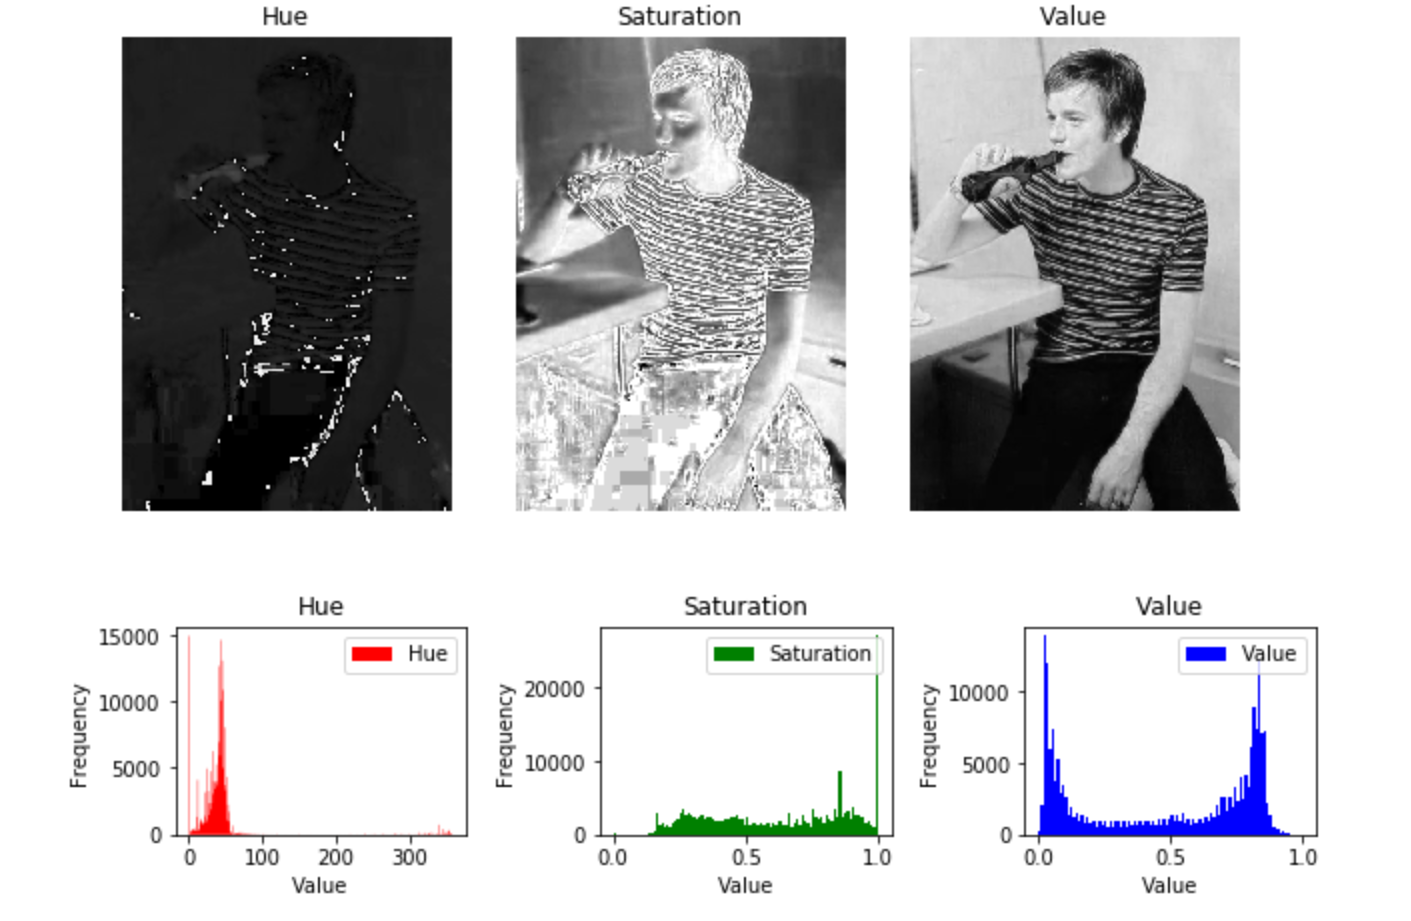
\includegraphics[width=1.0\textwidth]{hsv_histogram.png}
  \caption{左:H通道灰度图谱和颜色直方图;中:S通道灰度图谱和颜色直方图;右:V通道灰度图谱和颜色直方图}
  \label{fig:hsvhistogram}
\end{figure}

\subsubsection{局部二值模式}

  局部二值模式(Local Binary Pattern,LBP)是一种用来描述图像局部纹理特征的特征描述子,具有旋转不变性和对光照变化不敏感等优点,由\citet{ojala1994performance}在1994年首次提出。

  LBP的计算方法非常简单。每个像素都与它相邻的八个像素按指定的顺序(如顺时针、逆时针)作比较,来确定其特征值。对于中心像素大于某个相邻像素的,该像素对应的二进制位设置为0,否则设置为1,比较了中心点相邻的八个像素后,就得到了一个8位的二进制数,这个数字即为中心像素的特征值,计算过程如图\ref{fig:lbp_procedure}为例。图\ref{fig:lbp}为对图\ref{fig:ewan}的灰度图上的每个像素计算LBP值得到的LBP图谱,可以看出,LBP特征受噪点影响较重,能够突出表现物体的表面纹理,也能在一定程度上表现出物体的边缘。

\begin{figure}[htb]
  \centering
  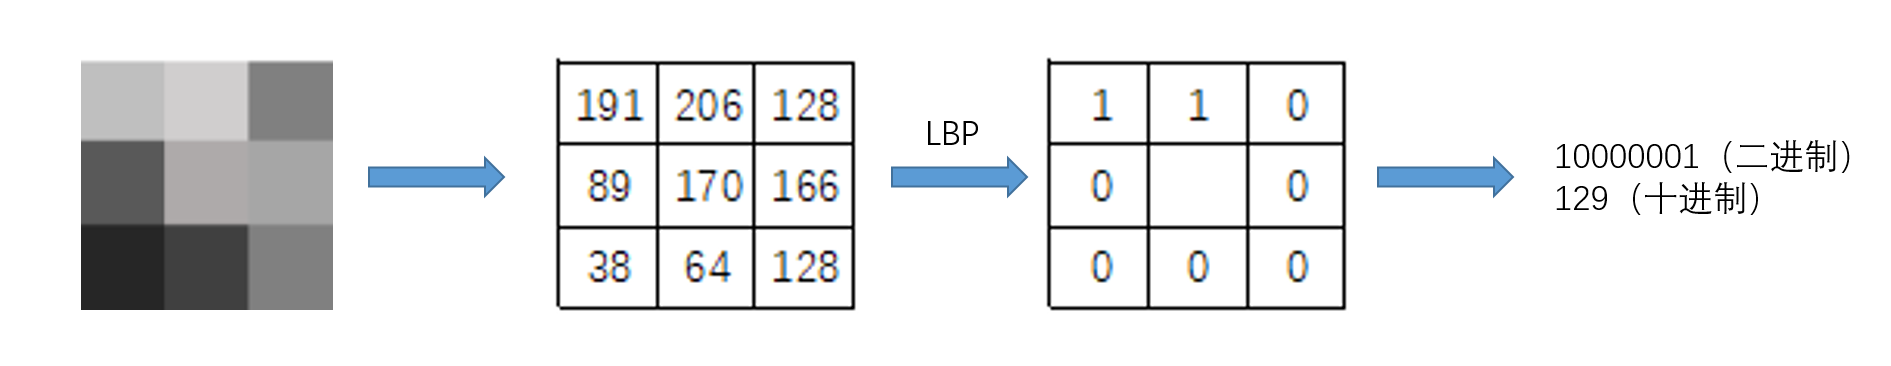
\includegraphics[width=0.9\textwidth]{LBP.png}
  \caption{计算3x3像素块中中心点的LBP值}
  \label{fig:lbp_procedure}
\end{figure}

\begin{figure}[htb]
  \centering
  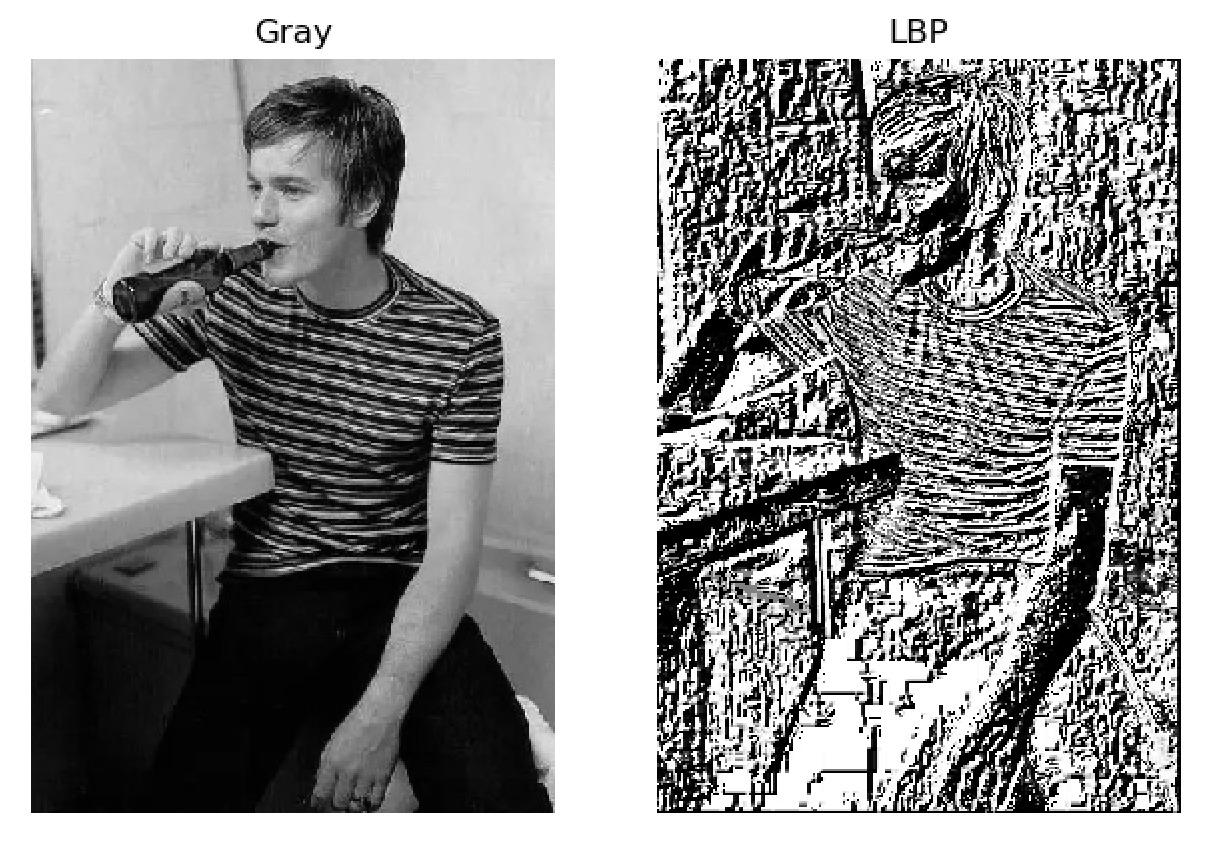
\includegraphics[width=0.6\textwidth]{ewan_lbp.png}
  \caption{左:灰度图;右:由灰度图计算得到的LBP图谱}
  \label{fig:lbp}
\end{figure}

  为了使得LBP描述子有旋转不变性,\citet{ojala2002multiresolution}提出了一个LBP的具有旋转不变性扩展方法,即不断旋转其邻域,得到一系列的LBP值,取其最小值作为该点的局部二值模式值。

  在计算一个图片的LBP描述子时,首先将图片分成固定大小的单元格(如$16\times16$像素),在计算出每个像素的LBP值后,统计每个单元格内的LBP值直方图,再串联所有单元格的直方图,即可得到该图片的LBP特征向量。

\subsubsection{方向梯度直方图}

  方向梯度直方图(Histogram of Oriented Gradient, HOG)是目前行人识别中最广泛使用的特征描述子之一。\citet{dalal2005histograms}在2005年提出了由HOG特征结合SVM分类器进行行人检测的方法,在此之后,该方法被广泛应用到了图像识别领域中,并尤其在行人检测中获得了巨大的成功,也出现了很多改进和变体。

  HOG特征描述算法通过计算和统计图像局部区域的梯度方向来构成特征。由于在物体的边缘和角落处图片的颜色会进行突变,故在这些区域,梯度的幅值也会变大。一般来说,边缘和角落比起平坦区域包含更多关于物体形状的信息,而通过对边缘和角度的描述,HOG正可以很好地描述局部目标的表面质地和形状信息。但同时,由于梯度的性质,HOG特征描述子对噪点比较敏感,且由于HOG主要描述了物体的轮廓,所以很难处理遮挡问题。

  为了计算方向梯度,我们可以简单地使用核向量(kernel)$[-1,0,1]$和$[-1,0,1]^{T}$对原图进行卷积,分别得到横向和纵向上的有向梯度。除了这种方法之外,还可以使用$[-1,1],[1,-8,0,8,-1]$和Sobel算子等作为核向量,不过根据\citet{dalal2005histograms}的实验,使用最简单的$[-1,0,1]$进行计算的梯度,在以HOG为特征进行的图像识别中效果反而最佳。

  在每个像素处,方向梯度都具有大小和方向。对于彩色图像,我们分别计算RGB三个通道的梯度。对原图片上的每个像素点$(x,y)$,$f(x,y)$为其R、G、B值中的一个,该通道上的横向和纵向方向梯度为:
\begin{gather*}
g_x(x,y)=[-1,0,1]\ast f(x,y)=-f(x+1,y)+f(x-1,y),\\
g_y(x,y)=\begin{bmatrix}
-1 \\
0 \\
1
\end{bmatrix}
\ast f(x,y) = -f(x,y+1)+f(x,y-1)
\end{gather*}

  由此便可得到有向梯度的幅值和方向:
\begin{gather*}
|g(x,y)|=\sqrt{g_x (x,y)^2 + g_y (x,y)^2} \\
\theta (x,y)=\tan^{-1}\left(\frac{g_y(x,y)}{g_x(x,y)}\right)
\end{gather*}
  
  使用以上公式在RGB颜色空间上计算图\ref{fig:ewan}的梯度值大小,如图\ref{fig:gradients}所示。可见,这张梯度图谱已经省略了图中很多不必要的信息,如颜色几乎一致的背景等,且突出了人物的轮廓、五官、衣服的图案等用于识别的重要信息。

\begin{figure}[htb]
  \centering
  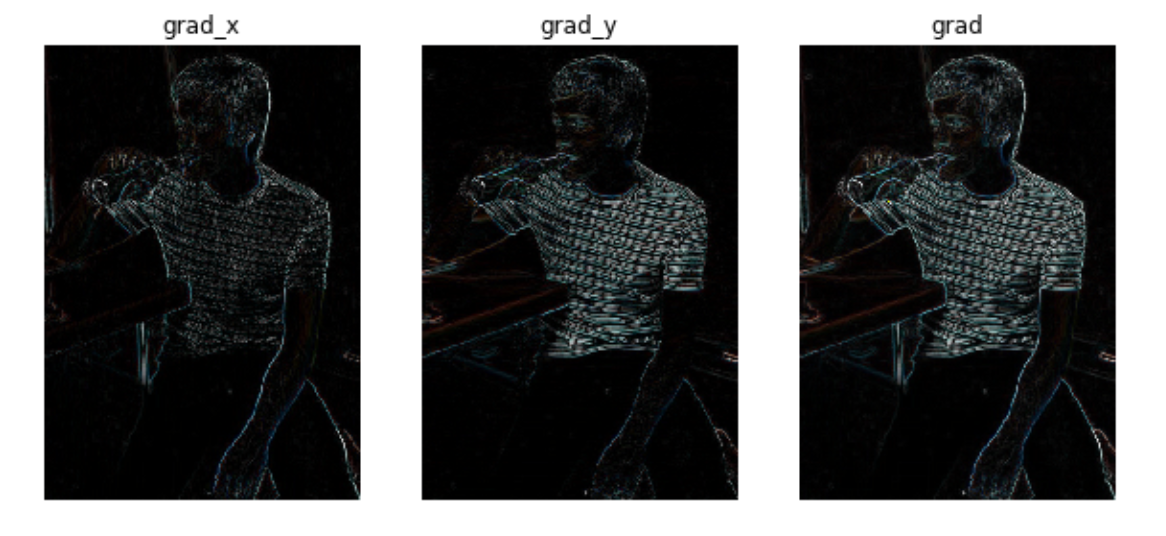
\includegraphics[width=0.9\textwidth]{gradients.png}
  \caption{左:横向梯度绝对值;中:纵向梯度绝对值;右:梯度大小}
  \label{fig:gradients}
\end{figure}

  此时在每个像素上得到的梯度有3个,分别对应原图的RGB分量,在计算HOG特征向量时,我们选取这三个通道的梯度幅度的最大值作为该点处的梯度大小,最大值对应的通道的梯度角度为该点处的梯度方向。

  方向梯度直方图统计的即为梯度大小为权重的梯度方向。梯度的方向范围为$[0^{\circ},360^{\circ})$,但是我们实际在统计方向时,采用的却是$[0^{\circ},180^{\circ})$的统计范围,通过计算$\theta(x,y) \mod 180^{\circ}$来代替原有的角度值,即把相差$180^{\circ}$的两个角度视为同一个梯度方向。实验表明,这种统计方式得到的结果往往比采用$[0^{\circ},360^{\circ})$范围的原方向效果更好\cite{dalal2005histograms}。

  值得注意的是,由于图像的梯度是由各像素点周围的颜色值大小计算得到的,所以也会受光照的影响,例如,将所有像素值除以2来使图像变暗,这时所有梯度大小也会随之减半,梯度直方图每个bin的高度也会减半。而在一张图片中,每个局部区域的光照可能会有所不同,为了降低这些影响,在进行方向梯度统计时,并不会直接统计一整个图片的方向梯度直方图,而是以$8\times8$像素的区域为一个单元格(cell)来分别进行统计,再在此基础上进行规范化(normalization)。这样会降低光照等噪音对特征描述子质量的影响,使HOG描述子更加稳定鲁棒。这个过程可以图\ref{fig:procedure}为例。

\begin{figure}[htb]
  \centering
  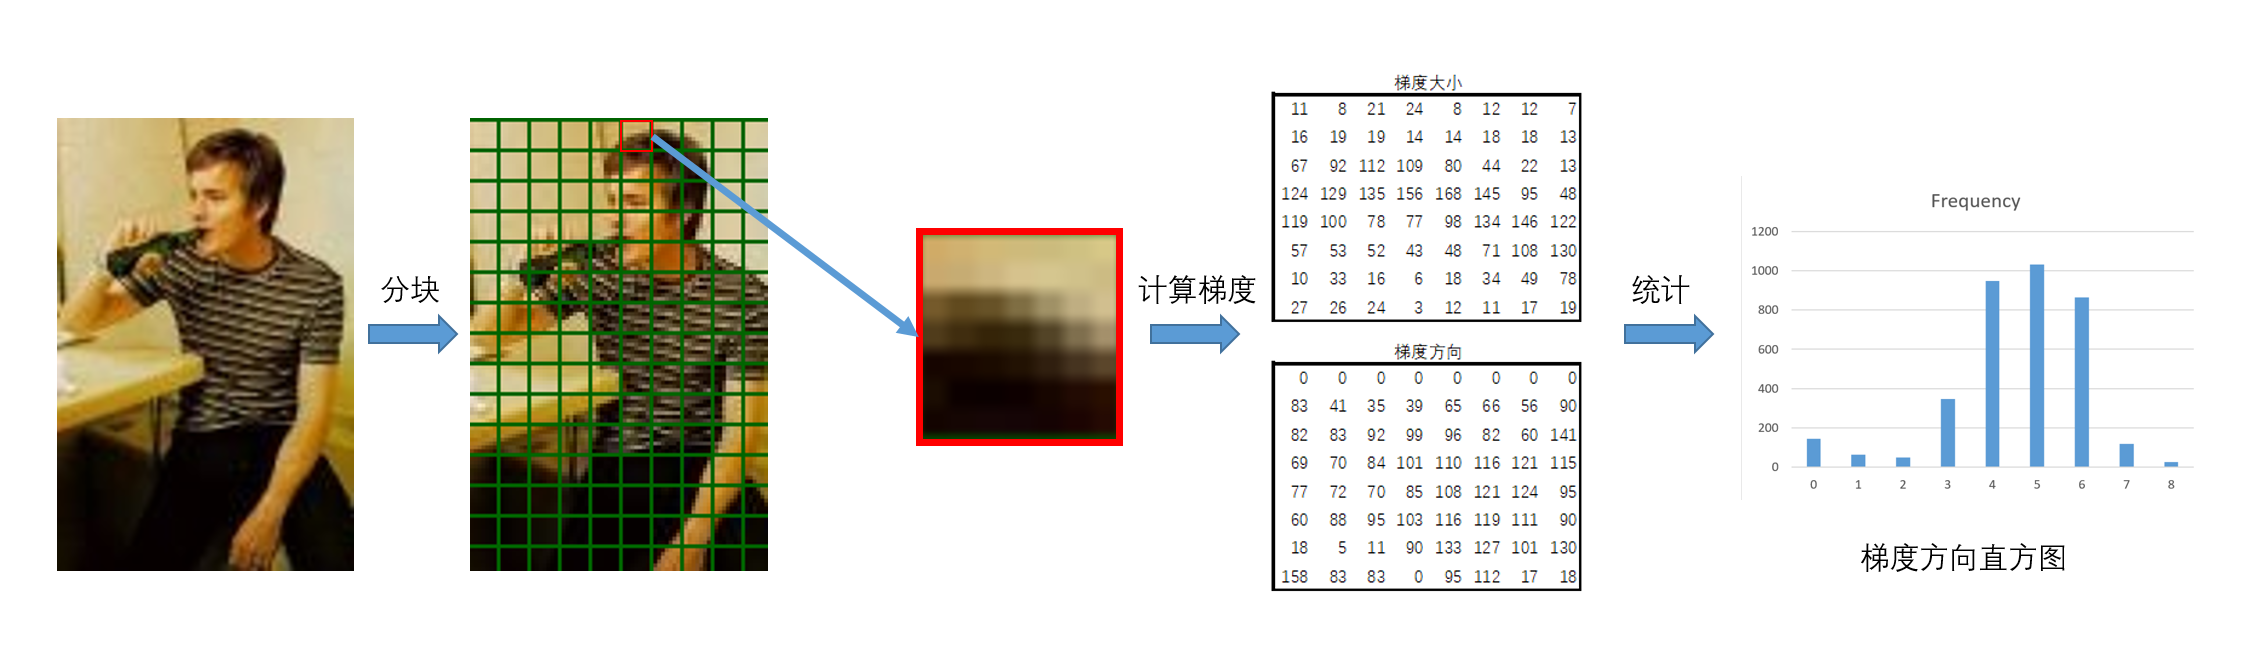
\includegraphics[width=1.1\textwidth]{procedure.png}
  \caption{统计单元格梯度直方图的过程示意图}
  \label{fig:procedure}
\end{figure}

  在进行规范化时,最常用的方法是在单元格的基础上取一个更大的块(block),每块的大小为$16\times16$像素,即包括4个单元格,将每一个块的4个HOG向量作为一个整体进行L2规范化。即$\vec{v}\leftarrow\vec{v}/\sqrt{\lVert v \rVert^2_2 + \epsilon^2}$,其中$\epsilon$是一个防止零除的足够小的正常数。以每个直方图取9个bins为例,在规范化一个块之后,我们得到了一个长为$4\times 9=36$的向量,即这个块最终的HOG向量。再以8像素的步长(stride)移动这个块,对下一个块进行规范化,即两个相邻块之间有2个单元格的重叠。如此循环,直到整张图的每一个单元格都被计算,再将所有经过的块的向量合并在一起,作为整张图的HOG描述子。

\subsubsection{尺度不变特征变换}

  尺度不变特征变换(Scale-invariant feature transform,SIFT)是一种不受图片尺度和旋转影响,并在一定程度上不受光照和相机视角影响的特征描述子,它将图像数据转换为有关局部特征的尺度不变坐标。同时,通过在空间和频率域的准确定位,SIFT还可以减少遮挡和噪音带来的干扰。SIFT可以使用有效的算法从图片中提取出大量的独特特征,可以在几乎所有尺度和位置上密集地覆盖图像,例如,一个$500\times500$像素的图像可以最多生成2000个稳定的特征点。SIFT算法中独特的关键点描述方法,可以使单个特征从大型特征数据库中能得到高概率的匹配。但在较为杂乱的图像中,背景中的很多特征可能会生成错误的匹配,不过通过识别关于目标物及其在新图像中的位置,尺度和方向的关键点的子集,可以从完整匹配集中过滤出正确的匹配\cite{lowe2004distinctive}。

  为了最大限度地降低提取特征的计算量,SIFT使用级联过滤(cascade filtering)方法来检测关键点,先使用高效的算法使用弱分类器检测出一些侯选位置,然后再进一步详细检测,将更加耗时的计算只在通过了初始测试的候选点位置上进行。但即使如此,SIFT特征描述子的计算量仍难以在行人检测和追踪中满足实时性要求\cite{zhou2009object}。故虽然SIFT特征描述子虽有诸多非常好的特性,但在有实时性要求的行人检测和追踪中并不常被使用。

\subsection{分类器}

  分类器的作用是通过拟合一个从样本到标签的映射函数,将图像中的区域分类为目标对象或背景。分类器的训练需要正负样本,分别对应目标区域和背景区域。在对分类器进行一定规模的训练后,此时将一个图像上的区域块的特征向量作为分类器的输入,分类器即会给出该区域包含目标物体的概率。

  在实际使用时,得到了一个图像帧后,选取不同的检测窗口的大小,即尺度,然后以给定尺度的检测窗口扫描整个图像,计算每个检测窗口的特征向量,使用分类器得出其中包含目标物的概率,如果这个概率超过给定的阈值,则认为该检测窗口中即包括待追踪物体。

\subsubsection{最近邻算法}
  常用追踪器TLD中便采取了最近邻算法(K-Nearest Neighbors)作为级联分类器的最后一级。KNN算法是从已有正确标签的样本集合中,找出与待分类特征向量最近的$k$个向量,以其中的多数的类别来决定该待测特征向量的分类。KNN算法的思想非常简单,一般使用欧式距离或巴氏距离作为向量间距离的度量,但随着样本集变大,计算$k$个最近邻的计算量也会很大,变得相当耗时,此外,它对数据的局部结构也非常敏感,也没有考虑不同分量的权重。

\subsubsection{随机森林}
  随机森林是一个包含多个决策树的分类器。决策树作为常用的机器学习方法有其缺陷,即训练时容易出现过学习,在训练集上具有低偏差和高方差的特点。而随机森林将多个深决策树的结果进行平均以降低方差,每个深决策树都在一个数据集上的不同部分进行训练,由此提高决策树的性能。事实上,随机森林分类器和K近邻分类器十分相似,都可以被看作是“对邻居向量结果的加权”。与KNN算法不同,随机森林在决定类别时可以评估各个分量的重要性,且对于不平衡的分类数据集,可以平衡误差,学习过程也较为快速。但随机森林仍然存在过拟合的问题,对于取值划分较多的分量上评估的权值偏大。

\subsubsection{支持向量机}

  支持向量机(Support Vector Machine,SVM)是一个监督学习的分类器。为了减少计算量,在用于行人识别时,一般采用线性支持向量机。它在特征空间中通过训练拟合一个最优超平面,在预测时通过将样本和最优超平面进行比较,判断它出现在某一类别的概率。对于线性不可分的样本,通过使用非线性算法将数据从低维空间转化到高维空间使其线性可分,再从高维空间采用线性回归。

  SVM对于在线学习的支持并不算好,通常只在初始化时进行对模型的拟合。

\subsubsection{AdaBoost}

  由于SVM计算量较大,为了提高速度,也可以使用AdaBoost代替。AdaBoost是Boosting分类器的一种,即一种由几个弱分类器组成的级联分类器,每一个弱分类有一个权重,结合起来就是一个强分类器。每一级分类器都会排除一些可能性较低的背景窗口,留下一些候选窗口传入下一级分类器进行计算。这样一来,在计算时大部分背景窗口在开始的几级分类器中就会很快被排除掉,剩下的很少一部分候选区域再通过后续的分类器,这样可以很大程度上提高整体运行速度。这里的弱分类器可以使用分类回归树、朴素贝叶斯模型、决策树桩等。

  在训练初始化时,AdaBoost给训练集的每个样本指定一个相同的权重,表明在训练时选取该样本进行学习的概率,接着调用弱分类器进行迭代学习,每次迭代后更新训练集上样本的权重,对于训练失败的样本赋予更大的权重,这样就使得下一轮的训练中,能够聚焦于那些更加难以分类、更富信息的样本上。


\section{基于动态的追踪}

  在基于动态的追踪中,我们假定在此前的几乎所有帧中都已成功地跟踪了对象,并保有对其运动模式和之前位置的记录,目标是根据这些已有信息找到在当前帧中物体的位置。物体的运动模型给了一个它当前位置的粗略预测,此外,还需要根据该目标对象在先前的帧中的外观记录(即特征)对物体的位置进行更加精确的估计,我们仍可以使用在目标检测中提过的物体特征,如颜色直方图,HOG等。根据这些外观的模型和特征,我们可以在由物体运动模型所预测的物体位置的邻域中进行搜索,以提高速度和准确度。根据外观进行分类的原理与目标检测相同,但如何将物体的运动模型等信息目标检测结合起来,就需要使用下面提到的几种算法。

\subsection{Boosting算法}
  在目标追踪中,我们常使用在线分类器进行目标识别,即在运行时即使训练的分类器。分类器的训练过程中,最初的正样本由使用者提供,在一张包含目标人物的图像中手动或使用某种检测算法选出一个框(bounding box,bbox)。分类器将该图像中的bbox作为正样本,在bbox之外取出若干个负样本进行训练拟合。

  在收到下一帧后,在物体原位置的所有相邻的位置上运行分类器,取得分最高的一个bbox作为当前帧的物体位置,再以当前帧检测出的bbox作为正样本,背景中提取负样本继续训练分类器。Boosting算法原理非常简单,相应地,追踪效果也比较平庸,由于它每次会选择得分最高的位置作为当前帧的检测结果,可能并不能选取到正确的目标位置,且容易出现漂移现象。

  在Boosting算法的基础上,\citet{babenko2009visual}提出了多示例学习(multiple instance learning,MIL)算法。不同于传统的分类器将每一个实例进行分类的方法,MIL将若干个实例归到一个包(bag)中,即正样本包和负样本包。只要包中的一个图像是正样本,就将其认为是正样本包,相对的,只有包中所有实例均为负样本,才将其认为是负样本包。构建正样本包的方法是首先包含目标物在当前图像中的图像块,并以此为中心,将该位置周围的小邻域中的图像块都包括其中。这样以来,即使被跟踪对象的当前位置不准确,只要将目标物作为中心的图像块被作为邻域放入了正样本包中,分类器就可以以它进行训练。

  但Boosting和MIL算法都有着共同的缺点,它们难以判断出是否已经对目标物失去了追踪而错误地选定了其他位置,此外,当目标物在一段时间内被遮挡的情况下,它们都难以恢复追踪。

\subsection{卡尔曼滤波}

  卡尔曼滤波是一种假定目标物体的运动服从线性高斯分布,以此对目标的运动状态进行预测,将预测结果与观察模型进行比较,根据误差更新预测模型,估计物体的当前位置的方法。它不是单纯地在前一帧目标物位置周围作检测,而是主动对其运动状态进行建模,预测它即将出现的位置\cite{welch1995introduction}。
  
  卡尔曼滤波分为两组方程:时间更新方程和测量更新方程。时间更新方程根据当前状态和误差协方差估计,预测下一时间的先验估计;测量更新方程用于根据所获得的新的测量,再结合先验估计来获取一个已优化的后验估计,这个后验估计又被传回时间更新方程。如此循环,完成一个预测-矫正的过程,以自动化地对模型进行更新,对状态进行估计。

  时间更新方程包括:
\begin{gather*}
\hat{x}^{-}_{k+1}=A_k \hat{x}_k + B u_k \\
P^{-}_{k+1}=A_k P_k A^T_k + Q_k
\end{gather*}

  测量更新方程包括:
\begin{gather*}
K_k=P^{-}_k H^T_k(H_k P^{-}_k H^T_k + R_k)^{-1} \\
\hat{x}_k = \hat{x}^{-}_k + K (z_k - H_k \hat{x}^{-}_k) \\
P_k = (I-K_k H_k)P^{-}_k
\end{gather*}

  $Q_k$和$R_k$均为常数,分别与$w$和$v$相关,估计误差协方差$P_k$和增益矩阵$K_k$将会在计算中迅速收敛,并保持不变。

  卡尔曼滤波器限定了系统噪声必须符合正态分布,且必须为线性系统,而在实际使用中,很难同时满足要求,此时精度就会较低。

\subsection{粒子滤波}

  粒子滤波器(particle filters)是一种基于概率密度的粒子表示的顺序蒙特卡洛方法(sequential Monte Carlo methods),它可以应用在任意状态-空间模型,可以对非线性、非高斯系统的动态进行建模,是传统的卡尔曼滤波的一般化方法\cite{arulampalam2002tutorial}。

  首先对跟踪目标进行建模,并定义一种相似度度量确定粒子与目标的匹配程度。在目标搜索的过程中,它会先按照一定的分布(比如均匀分布或高斯分布)在全局撒一些粒子,统计这些粒子与目标的相似度,确定目标可能的位置。

  首先在目标周围均匀地或按高斯分布随机散布一些粒子,它们在图中的位置分别为$\{x_i,i=0,\dots,N\}$,每个粒子都计算其所在区域内的特征向量,与初始的目标区域的特征作比较,得到一个相似度,将这些相似度归一化得粒子的权重$\{w_i,i=1,\dots,N\}$,$\sum_{i=1}^N w_i = 1$。则在这张图像上,目标最可能在位置为$\sum_{i=1}^N w_i x_i$。之后,我们根据每个粒子的权重$w_i$进行粒子重采样,在概率较大的位置多撒粒子,减少概率小的位置的粒子个数,将重采样后得到新的粒子集再通过顺序重要性采样算法(Sequential Importance Sampling)得到新的粒子集,用于下一帧的目标识别。

  粒子滤波器相对于卡尔曼滤波器,虽然适用范围更广,但计算量也更大。

\subsection{均值漂移算法}
 
  均值漂移算法(MeanShift)是用于定位图中概率密度最大的位置的算法,常常结合HSV颜色直方图进行目标跟踪。以利用HSV颜色直方图模型为例,给定了一个初始的包括目标行人的搜索窗口,MeanShift算法首先将图片的RGB分量转化为HSV分量,统计该搜索窗口内的H分量直方图,将直方图归一化后,我们便可以得到所有H值($\in [0^{\circ},360^{\circ}]$)对应的概率。在统计直方图时,为了避免由于低光照导致的错误数据,将V值低于某一阈值的像素点不予统计。接着,将全图的所有像素值都用它的H分量所对应的概率表示,得到的图像被称为反向投影图,如图\ref{fig:backproject}所示。MeanShift所谓的求图中概率密度最大的位置,即是求反向投影图中平均值最大的窗口,在CamShift中用一种类似梯度下降法的方法实现,求得局部最大值。对于新的一帧,首先求当前搜索窗口的质心位置,即将像素概率作为权重,求所有位置的加权平均,接下来将这个质心作为新的搜索窗口的中心,重复计算其质心,如此循环,直到搜索窗口收敛,即为概率密度的局部极大值。

\begin{figure}[htb]
  \centering
  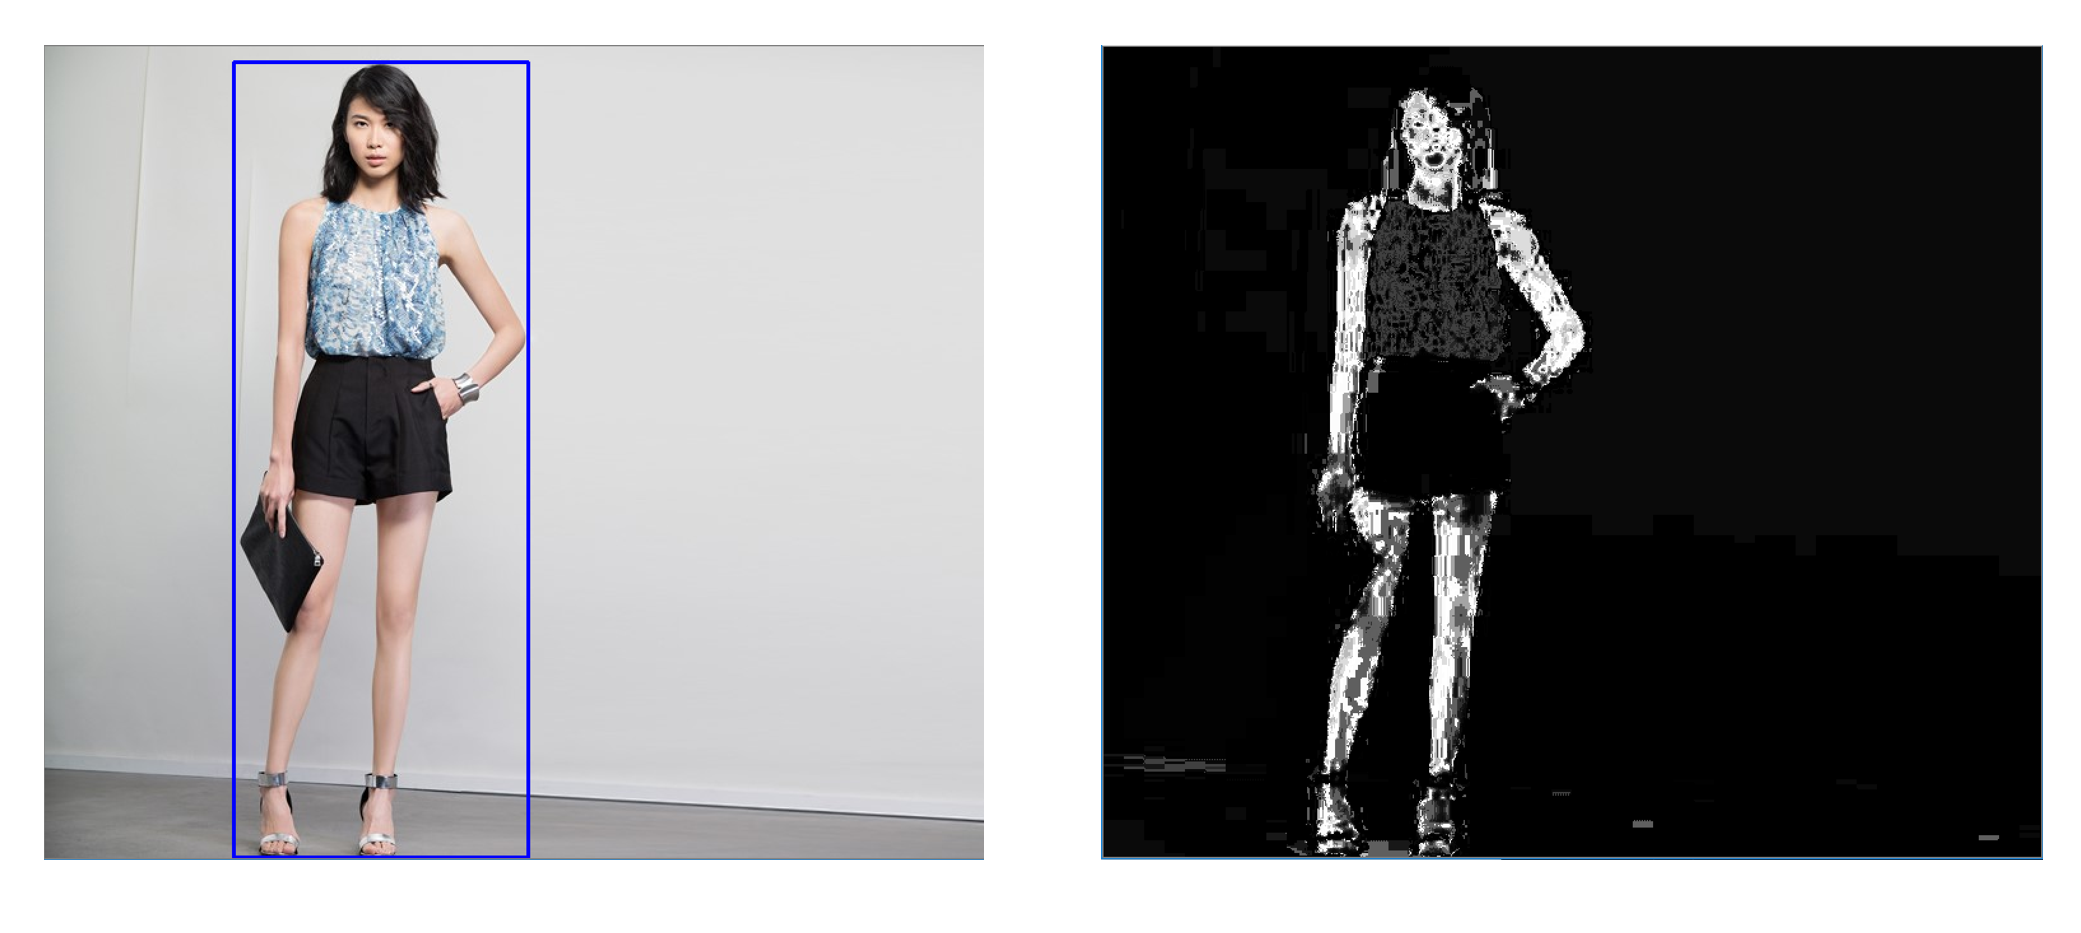
\includegraphics[width=0.9\textwidth]{backproject.png}
  \caption{左:原图像,蓝色框内为初始提供的含目标行人的搜索窗口;右:反向投影图}
  \label{fig:backproject}
\end{figure}

  在MeanShift算法的基础上,\citet{bradski1998computer}提出了一种对MeanShift算法在视频上的扩展,即连续自适应均值漂移算法(Continuously Adaptive MeanShift,CAMShift)。CAMShift算法对视频的所有帧都进行MeanShift运算,并将上一帧得到的目标所在窗口中心和大小作为下一帧的初始搜索窗口。相对于MeanShift,它在所有帧上都重新按照上一帧所得到的窗口计算反向投影图,此外,在每一帧上,当MeanShift算法收敛后CAMShift算法都会根据目前搜索窗口中的像素概率值之和更新搜索窗口的大小,这样以来就可以一定程度上解决目标在尺度上的变化、形变和部分遮挡。

\subsection{相关滤波}

  在信号处理中,使用相关性来描述两个信号之间的联系。在相关滤波算法中,根据当前帧的信息和之前帧的信息训练出一个相关滤波器,然后与新输入的帧进行相关性计算,得到的置信图表示了输入帧中每个像素或图像块是目标的位置概率,得分最高的点或块就是最可能的跟踪结果。

  \citet{henriques2015high}在2015年提出了KCF算法(Kernelized Correlation Filters),它利用了在傅里叶域中,两个矩阵的卷积可以被转换为逐元素的点乘的性质,在达到与以往的更加复杂的算法的效果的基础上,降低了计算所需要的资源和时间。

  KCF算法中可以使用三种核函数,包括线性、多项式和高斯核函数,使用岭回归进行拟合以得到一个闭式解,都使用较少的计算量得出了较好的预测结果。它通过使用输入向量生成循环矩阵,一方面通过位移增加了样本的个数,一方面利用了循环矩阵可被离散傅里叶变换(DFT)对角化的特性,将岭回归中的求逆运算、矩阵乘法等转换为了计算量小的矩阵间逐元素计算,从而大大提高运行速度。

  由于KCF使用傅里叶变换,导致滤波器尺寸和图像块尺寸必须一致,这样就限制了检测的尺度,导致KCF算法对尺度变化的适应性不强,当物体在图像中的尺度发生变化时,会导致KCF算法不能正常地对物体进行追踪。此外,KCF使用循环矩阵虽然可以增加分类器的样本数量,但也导致了有些训练数据并不真实。为了解决这些问题,\citet{lukezic2017discriminative}在2017年提出了通道和空间稳定的判别性相关滤波器(Discriminative correlation filter with channel and spatial reliability,CSR-DCF)。根据实验,它有着比KCF算法更高的精度,相对的,帧率较KCF更低。

  CSR-DCF算法通过引入空间置信度和通道置信度来对相关滤波器做出改进。空间置信度图是由反向投影图和先验概率得到每个像素点是目标的后验概率经过二值化后得到的。空间置信图可以用来修正追踪器的尺度,且可以有效地帮助追踪非矩形的区域或目标。

  定义对第$i$个像素点的观察$y_i=[y_i^c, y_i^x]$,分别表示该像素的颜色和位置,$m_i$为该像素点空间置信度,则$y_i$的概率为:
$$p(y_i)=\sum_{j=0}^1 p(y_i^c | m_i=j)p(y_i^x | m_i=j)p(m_i=j)$$

  其中$p(y_i^c | m_i=j)$为由背景和前景的颜色直方图根据贝叶斯规则得到,类似于Mean-Shift中的方法,根据像素的颜色名计算反向投影图,得到各像素点属于前景或背景的概率。$p(m_i=j)$为该像素属于前景或背景的先验概率,由前景和背景的区域大小比例决定。估计的目标位置的中心像素即使在旋转、变形等情况下仍然很大可能含有目标,而在没有测量的情况下,远离中心的像素属于目标和背景的概率是相当的。基于这些知识,可以通过Epanechnikov核函数估计的弱空间先验概率:
$$p(y_i^x | m_i=j) = k(x;\sigma)=1-(x/\sigma)^2$$

  其中$\sigma$是最小界限框的轴长,此外,先验概率被限制在$[0.5,0.9]$的范围内,即在中心点周围的像素先验概率为0.9,当像素离中心越远时,先验概率越小,而远离中心点的像素,先验概率均为0.5。通过先验概率和颜色置信度计算出空间置信度图再进行二值化后,由于其中的元素由0和1组成,故通过将它和滤波器进行点乘,就可以排除掉图像中空间置信度为0的点。在加上这个空间限制后,无法得到一个滤波器的闭式解,但可以通过迭代的方法最小化损失函数,得出滤波器的值。在追踪的过程中,一旦目标被定位,滤波器也会根据提取出的区域进行更新。

  通道置信度反映了每个特征通道对应的滤波器的辨别能力和重要性,在目标定位阶段计算相关响应时将其作为每个滤波器的权重,包括了通道学习置信度和通道检测置信度。

  CSR-DCF算法的每一次迭代都分为定位和尺度估计,以及更新两个阶段。在定位和尺度估计阶段,根据上一帧的图像块特征、滤波器和通道置信度的相关响应最大值得到一个新的目标位置,根据各通道的响应,估计新的通道检测置信度,使用新的位置根据DSST算法来估计尺度。在更新阶段,提取前景和背景的颜色直方图,并估计空间置信图,更新滤波器和通道置信度。

  CSR-DCF算法在速度和准确度上都达到了非常好的水平,在单CPU上既能达到实时,在准确度上,CSR-DCF算法在VOT2017比赛的实时实验部分取得了最佳结果\cite{kristan2017visual}。

\subsection{GOTURN}

  GOTURN是一个基于深度神经网络的跟踪算法\cite{held2016learning},在深度学习的跟踪算法中,GOTURN由于其达到100FPS的高帧率脱颖而出,它对于视角的变化、光照、变形等具有鲁棒性,但不能很好地处理遮挡。

  GOTURN网络以视频当前帧和上一帧作为输入,输出当前帧的目标所在区域的bounding box的位置。GOTURN的网络结果如图\ref{fig:GOTURN}所示。其中的卷积层(Conv Layers)用于抽取图像特征,全连接层(Fully-Connected Layers)用于特征比较,找出当前帧上的目标位置。上一帧的剪切(crop)已知,当前帧的剪切是以上一帧的跟踪目标为中心,截取两倍目标大小的区域作为搜索区域,在该区域内进行回归。

\begin{figure}[htb]
  \centering
  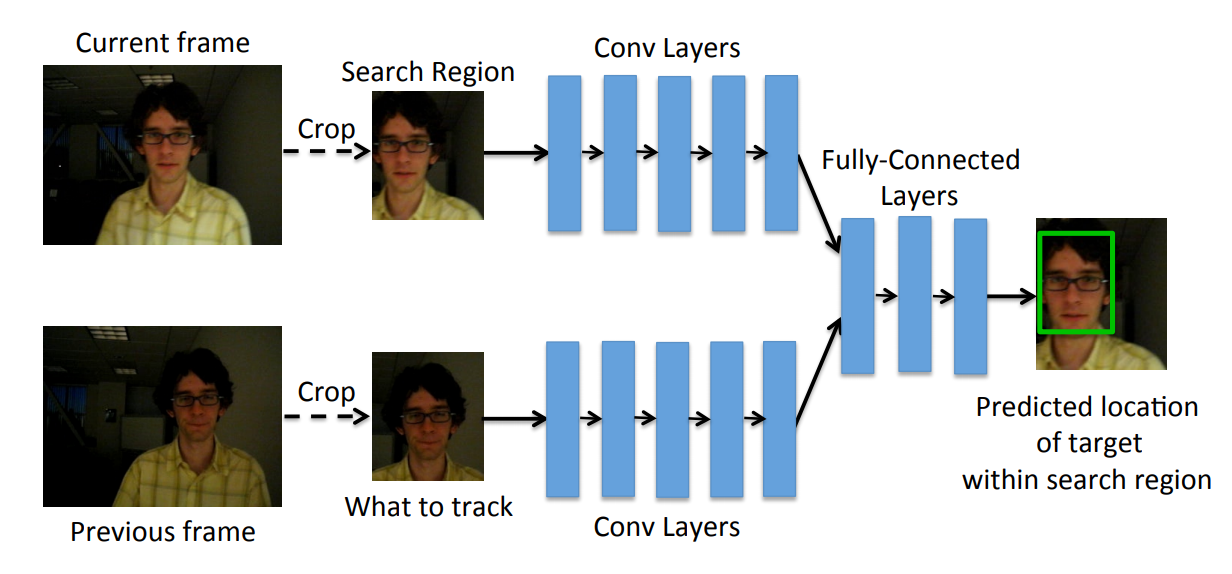
\includegraphics[width=0.9\textwidth]{GOTURN.png}
  \caption{GOTURN神经网络结构}
  \label{fig:GOTURN}
\end{figure}

\subsection{TLD}

  TLD,即Tracking-Learning-Detection是一种单目标长时间的目标追踪算法,TLD算法将长期追踪的任务分解成三个:跟踪、学习和检测。追踪模块在每个帧上不停地追踪对象的位置;探测模块在适当是时候对追踪其进行校正;TLD中还提出了P-N学习模块来识别检测器的错误并更新检测器,\cite{kalal2012tracking}。

  TLD中使用Median-Flow作为追踪器,使用窗口扫描法和级联分类器作为检测器。级联分类器分为三个阶段:图像块方差(patch variance)、集合分类器(ensemble classifier)和最近邻(nearest neighbor)。

  图像方差分类器计算目标物所在图像块的灰度值方差,并丢弃所有灰度值方差少于其50\%的待测图像块。50\%这一阈值可以根据具体应用调整,它限制了目标的最大外观变化。通过图像方差分类器的图像块再经过集合分类器,它由$n$个基本分类器组成,每个集合分类器$i$对图像块进行像素比较,并得到一个二进制码$x$,由$x$得到一个后验概率$P_i(y|x)$,其中$y\in\{0,1\}$。将每个基本分类器的后验概率进行平均,并将$y=1$的后验概率小于50\%的图像块舍去。最后一级分类器是最近邻分类。

  对一帧的探测和追踪都完成后,TLD取追踪器得到的目标所在边界框(bounding box)和探测器得到的边界框中置信最大的结果作为最终估计,当二者都没有得到边界框,则认为目标在这一帧中不可见。由于TLD不是一直采用追踪器的结果,所以边界框在帧之间可能会发生跳动。

\begin{figure}[htb]
  \centering
  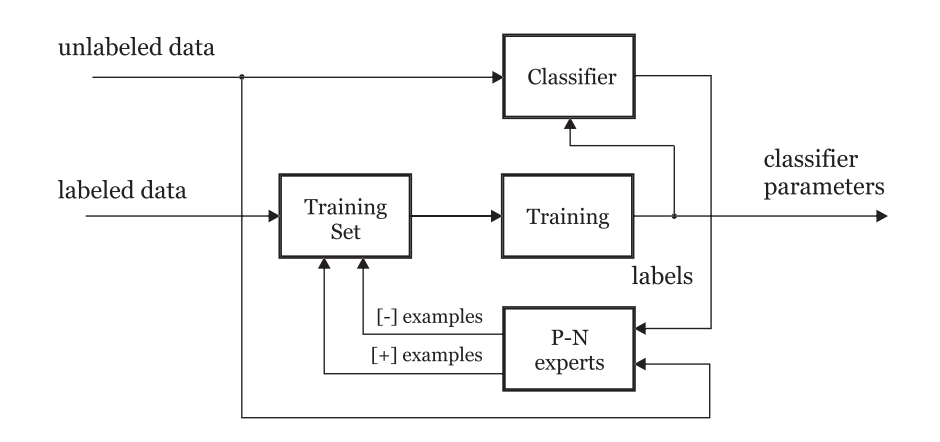
\includegraphics[width=0.9\textwidth]{tld.png}
  \caption{TLD学习模块结构}
  \label{fig:tldlearning}
\end{figure}

  学习模块是TLD算法的新颖之处,它在第一帧进行初始化,并在运行时更新探测器以改善其性能。学习模块分为四个部分:待训练的分类器、训练数据集、监督学习、P-N专家,如图\ref{fig:tldlearning}所示。P-N专家(P-N experts)用于在运行时生成训练所需的正样本和负样本并识别检测器的错误,P专家识别检测器的漏报(false negatives),并将其添加到具有正标签的训练集中,N专家识别被检测器预测为正的负样本(false positives),并将其添加到负标签的训练集中。此外,P专家还用于增加正样本的数量,当获得一个含有目标的界限框后,P专家将其通过几何变换生成若干个仿射的界限框,如将其进行$\pm 1\%$的偏移,$\pm 1\%$的尺度变换,$\pm 10^{\circ}$的平面内旋转等操作,这样可以通过增加正样本的数量来提高分类器的鲁棒性。N专家则通过在图像的界限框之外的区域取若干个图像块作为负样本。


  为了判断检测器的错误,P专家利用视频的时间连续性,记录目标的轨迹并假设目标延轨迹移动,由此预测当前帧中的目标物位置。如果检测器将当前位置标记为负,则认为是漏报,由P专家将其标记为正;N专家利用视频中的空间结构,并假设目标物在一帧中只能出现在一个位置,它分析当前帧中检测器和跟踪器产生的所有结果,选择置信度最高的结果,并将与所选界限框不重叠的图像块标记为负。需要注意的是,P-N专家所判断的错误并不总是正确的,它们的假设都有失效的情况,但尽管误差存在,P-N学习模块仍能够改善检测器的性能,即这种误差在一定条件下是允许的。
